%auto-ignore


\chapter{Graphical Calculus for Reshetikhin-Turaev graphs}
\label{cha:rt}

In this chapter we state (with no proof!) some results of graphical
calculus, as developed by Reshetikhin and Turaev in
\cite{reshetikhin-turaev;ribbon-graphs}, which are most relevant for
the simplified theory in \csref{cha:gc}. Infact, Reshetikhin-Turaev
graphs are rich enough in structure to accommodate the graphical
calculus on a category which is at a time braided, autonomous, and
tortile.

To avoid a clash of nomenclature, the ``ribbon graphs'' of Reshetikhin
and Turaev's \cite{reshetikhin-turaev;ribbon-graphs} have been renamed
``RT-graphs''. Also, the categorical terminology is chosen in
accordance with \csref{cha:btc} so is somewhat discordant with that of
Reshetikhin-Turaev's paper.

\section{The category of Reshetikhin-Turaev diagrams} 
\label{sec:rt-diagrams}

Let $L$ be the infinite strip $\setR \times [0,1]$; for $j \geq 1$ let
$s_j$, $t_j$ be the points $(j, 0) \in L$ and $(j,1) \in L$,
respectively.
\begin{definition}
  An RT-diagram $\Gamma$ of type $(p,q)$ is given by a finite set
  $\Vertices{\Gamma}$ (the set of vertices) and a finite set $\Edges{\Gamma}$
  (the set of edges) such that:
  \begin{itemize}%[RT1)]
  \item  each vertex $v$ is a tiny
    rectangle\footnote{Called a ``coupon'' in Reshetikhin-Turaev's
      original wording.} contained in the strip $L$ with two of its
    edges parallel to the boundary of $L$ --- call them
    $\text{Top}(v)$ and $\text{Bottom}(v)$;\label{RT1}
  \item each edge is a smooth immersion $\ell\colon[0,1]\to L$;\label{RT2}
  \item  for each $\ell\in\Edges{\Gamma}$, the \emph{endpoints}
    $\ell(0)$, $\ell(1)$ lie in \begin{equation*}\{s_1,\ldots, s_p\}\cup\{t_1,
      \ldots, t_q\}
      \cup\bigcup_{v\in\Vertices{\Gamma}}\bigl(\text{Top}(v)\cup\text{Bottom}(v)
      \bigr);\end{equation*} the points $\ell(0)$ and $\ell(1)$ are
    called the \emph{source} and \emph{target} of the edge $\ell$
    respectively;\label{RT3}
  \item  no two edges have a common endpoint;\label{RT4}
  \end{itemize}
  Moreover, $\Gamma$ comes equipped with the following data:
  \begin{itemize}
  \item for every crossing of edges (including self-crossings) an
    element in the set
    \begin{equation*}
      \left\{\, \xy*!LC\xybox{\vcross}\endxy \,,\, 
        \xy*!LC\xybox{\vcrossneg}\endxy \,\right\}
    \end{equation*}
    must be specified, that is, we want to know which of the two
    crossing arcs ``passes under'';\label{RT5}
  \item for every edge $\ell \in \Edges{\Gamma}$, an orientation
    (``direction'') of $\ell$ is chosen;\label{RT6}
  \item for every edge $\ell \in \Edges{\Gamma}$, a framing of $\ell$, that is,
    a map $N_\ell: [0,1] \to S^1$ is given, with the proviso that
    $N_\ell(0) = N_\ell(1) = 1$.\label{RT7}
  \end{itemize}
\end{definition}
We consider two framings $N_\ell$, $N'_\ell$ to be the same if they are
homotopic rel $\{0,1\}$. Thus, the framing data reduces to the
assignment of an integer number $n_\ell := \deg N_\ell$ to each edge $\ell
\in \Edges{\Gamma}$ (see \cite{shum;tortile-categories}).

When drawing an RT-diagram, we assume the \emph{blackboard framing},
that is, we choose the vector $N_\ell(t)$ to be the vector at $\ell(t)$
normal to the plane where $L$ lies and pointing upwards. When there is
need to consider another framing, we shall explicitly draw it.

A \emph{closed diagram} is a diagram of type $(0,0)$. Adding (or
removing) a connected component of type $(0,0)$ to a given diagram
does not change its type.
\begin{figure}[bhp]
\begin{equation*}
  {\xy
    ,(0,-1.5);(0.6,-0.4)*+[F]{\ }**\crv{(0,-1.3)&(0.4,-0.9)%
      &(0.6,-0.4)}?(.5)*\dir{>}%
    ,(0.6,-0.4)*+[F]{\ };(0.6,0.3)*+[F]{\ }**\crv{(0.6,-0.2)}%
    ?(.75)*\dir{>}%
    ,(0.6,0.3)*+[F]{\ };(0,1.5)**\crv{(0.5,0.5)&(0.4,0.7)}%
    ?(.85)*\dir{>}%
    ,(1.2,-1.5);(1.2,-1.1)*+[F]{\ }**\crv{(1.2,-1.3)&(1.2,-1.1)}%
    ?(.10)*\dir{<}%
    ,(1.2,-1.1)*+[F]{\ };(0.6,-0.4)*+[F]{\ }**\crv{%
      (0.8,-0.7)&(0.6,-0.5)}%
    ?(.5)*\dir{>}%
    ,(0.6,0.3)*+[F]{\ };(1.2,1.5)**\crv{(0.7,0.5)&(0.8,0.7)}%
    ?(.5)*\dir{<}%
    ,(1.2,-1.1)*+[F]{\ };(2,1.5)**\crv{(1.2,-1.1)&(1.4,-0.9)&(1.5,-0.7)}%
    ?(.85)*\dir{<},%
    ,(0,-1.7)*{+},(1.2,-1.7)*{-}%
    ,(0,1.7)*{+},(1.2,1.7)*{-}%
    ,(2,1.7)*{-},%
    ,(-0.2,-1.5);(2.2,-1.5)**\dir{-}%
    ,(-0.2,1.5);(2.2,1.5)**\dir{-}%
    \endxy}
\end{equation*}
\caption{An example of an RT-diagram with blackboard framing.}
\end{figure}

The projection $z\colon L \to [0,1]$ induces a differentiable function
$z\circ\ell \colon [0,1] \to [0,1]$ (the \emph{height function}) on every edge
$\ell\in\Edges{\Gamma}$.
\begin{definition}
Critical points of an RT-diagram $\Gamma$ are: 
\begin{inparaenum}
\item vertices, 
\item crossings,
\item critical values of the height function on every edge.
\end{inparaenum}
\end{definition}

\begin{example}
  A directed braid on $r$ strands can be seen as a diagram of type
  $(r,r)$ with no vertices and only crossings as critical points (and
  vice-versa).
\end{example}

If $v$ is a vertex of $\Gamma$, then let $\Leg(v)$ be the set of edges of
$\Gamma$ incident to $v$. Every set $\Leg(v)$ is divided into two
disjoint totally ordered subsets $\In(v)$ and $\Out(v)$:
\begin{equation*}
  {%
    \overbrace{\underbrace{\xy%
        (0,0)*{v},
        (0,1)*+[F]{\ };%
        (-1,0)**\dir{-},(-0.5,0)**\dir{-},(0,0.5)*{\ldots},(1,0)**\dir{-},%
        (-1,2)**\dir{-},(-0.5,2)**\dir{-},(0,1.5)*{\ldots},(1,2)**\dir{-},%
        \endxy}_{\In(v)}}^{\Out(v)}
    }
\end{equation*}

A sign $\varepsilon_x \in \{ \pm1 \}$ is given to each non-critical point $x$
belonging to an edge $\ell$, according to whether the chosen orientation
agrees ($+1$) or disagrees ($-1$) with the orientation pulled back via
the height function. This sign is locally constant (on edges except
critical points); by extension, a sign is unambiguously defined on
each source and target point; if $u$ is an endpoint, denote its sign
by $\sgn(u)$.
\begin{definition}
  The \emph{source} and the \emph{target} of an RT-diagram $\Gamma$ of
  type $(p,q)$ are the sequences of $\pm1$ given by
  \begin{align*}
    \Src(\Gamma) &\joinrel:= (\sgn(s_1),\sgn(s_2),\dots,\sgn(s_p)),
    \\
    \Tgt(\Gamma) &\joinrel:= (\sgn(t_1),\sgn(t_2),\dots,\sgn(t_q))
  \end{align*}
  For a vertex $v$ of an RT-diagram we can define $\Src(v)$ (resp.\ 
  $\Tgt(v)$) as the sequences of the signs of the endpoints of the
  edges in $\In(v)$ (resp.\ $\Out(v)$).
\end{definition}

\begin{definition}\label{dfn:graph-composition}
  Two RT-diagrams $\Gamma$ and $\Phi$ are \emph{composable} iff $\Src(\Gamma) =
  \Tgt(\Phi)$. If $\Gamma$ and $\Phi$ are composable, we can form a new
  diagram $\Gamma\circ\Phi$ by ``stacking $\Gamma$ on top of $\Phi$ and squeezing the
  stack to fit into $L$'' (see \csref{fig:graph-composition}).
\end{definition}
\begin{figure}[tbp]
  \begin{equation*}
    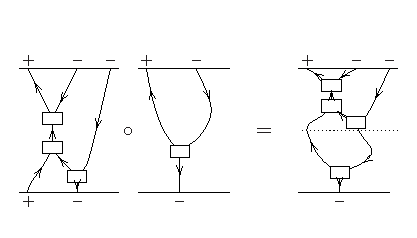
\includegraphics{fig-001}
  \end{equation*}
  \caption{Composition product of RT-diagrams.}
  \label{fig:graph-composition}
\end{figure}
\begin{figure}[tbp]
  \begin{equation*}
    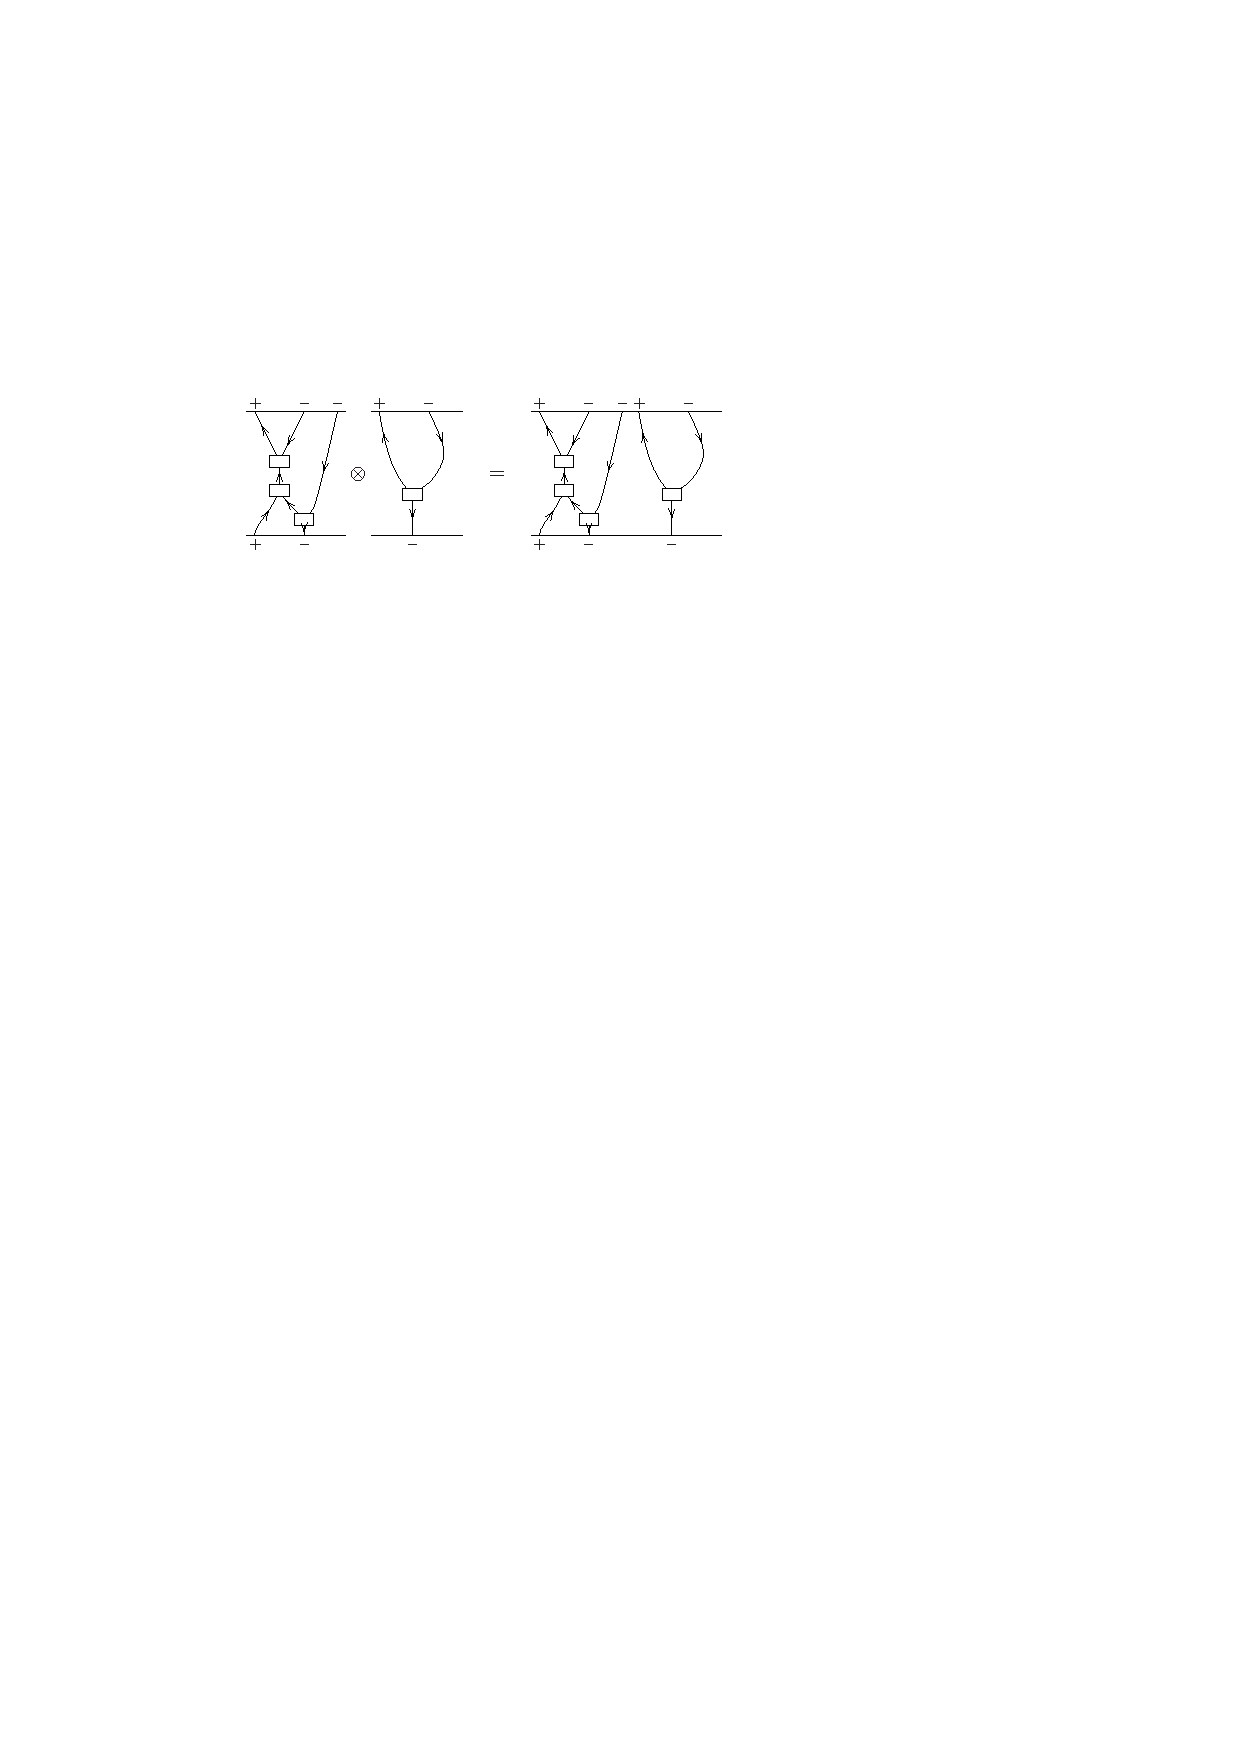
\includegraphics{fig-002}
  \end{equation*}
\caption{Tensor product of RT-diagrams.}
\label{fig:graph-otimes}
\end{figure}

Diagrams corresponding to directed braids on $n$  strands form a group
under the composition product, isomorphic to the semidirect product
$B_n \ltimes \setZ_2^n$.

By the above definitions, we can take the linear spans $\RTD(S,T)$ of
diagrams with given source $S$ and target $T$, as the $\Hom$-spaces of a
suitable category.
\begin{definition}
\label{dfn:diagrams-category}
$\RTD$ is the monoidal category which has finite sequences of $\pm1$ as
objects; the $\Hom$-space $\RTD(S,T)$ is the linear span of the set of
diagrams with source $S$ and target $T$.

Composition of morphisms is defined by bilinear extension of the
composition product $\circ$ (see \csref{dfn:graph-composition}).

The tensor product is given on objects by concatenation:
\begin{equation*}
  (\varepsilon_1, \ldots, \varepsilon_r) \otimes (\varepsilon'_1, \ldots, \varepsilon'_s) = (\varepsilon_1, \ldots, \varepsilon_r, \varepsilon'_1, \ldots, \varepsilon'_s),
\end{equation*}
and on morphisms by juxtaposition of diagrams (see
\csref{fig:graph-otimes}). 
\end{definition}

The category $\RTD$ is not braided, nor autonomous, nor balanced in
any obvious way: it is the deep result of Reshetikhin-Turaev
\cite{reshetikhin-turaev;ribbon-graphs}, Joyal-Street
\cite{joyal-street;tensor-calculus} and Freyd-Yetter
\cite{freyd-yetter;btc} that a quotient of it enjoys all these
structures; moreover, this result can be enhanced by considering
\emph{colored} graphs, and colors can be taken in any braided
autonomous tortile category.


\section{The category of RT-graphs}
\label{sec:rt-graphs}
Let $\Hom\RTD := \bigcup_{S,T \in \RTD} \RTD(S,T)$ be the set of all
morphisms in the category $\RTD$; $\Hom\RTD$ consists of all possible
RT-diagrams. Any RT-diagram can be considered as the planar projection
of a purely $1$-dimensional CW-complex equipped with some additional
structure.
\begin{definition}
  An (embedded) RT-graph\footnote{What is here called an ``RT-graph''
    corresponds to a ``homogeneous colored directed ribbon graph''
    (HCDR-graph) in the terminology of
    \cite{reshetikhin-turaev;ribbon-graphs}: the ``ribbon'' condition
    has been rephrased in terms of framing here, and the
    ``homogeneity'' is hidden in the requirement that $N_\ell$ satisfy
    $N_\ell(0) = N_\ell(1) = 1$. We do not need CDR-graphs (i.e., not
    homogeneous). Also, since we are ultimately going to consider
    coarser invariants than Reshetikhin and Turaev do, the definition
    of RT-graph has been adapted to suit a more combinatorial
    environment.} $\Gamma$ is a $1$-dimensional CW-complex embedded in $M
  = \setR \times [0,1] \times [0,1]$ together with
  \begin{itemize}
  \item for each edge, a choice of a direction;
  \item for each edge, a choice of a framing;
  \item for each vertev $v$, a partition of half-edges incident to it
    into disjoint totally-ordered subsets $\In(v)$ and $\Out(v)$.
  \end{itemize}
  In addition, we stipulate that $\Gamma \cap \partial M$ is a finite set --- call
  its points the \emph{endpoints} of $\Gamma$.  We say that $\Gamma$ has type
  $(p,q)$ iff $\Gamma \cap \partial M \subseteq \{ s_1, \ldots, s_p \} \cup \{ t_1, \ldots, t_q \}$.
\end{definition}
Extending a classical result of Reidmeister, Reshetikhin and Turaev
proved the following.
\begin{lemma}[\cite{reshetikhin-turaev;ribbon-graphs}]\label{lemma:moves}
  The set $\Hom\RTE$ of all isotopy classes (rel $\partial M$)\FIXME{Se
    dobbiamo considerare isotopie col bordo fisso allora non si pu{\`o}
    tagliare un grafo ad altezza generica\ldots vale la pena di essere
    estremamente precisi su questo punto?} of embedded
  RT-graphs is the quotient of the set $\Hom\RTD$ of RT-diagrams
  with respect to the equivalence relation generated by a finite set
  of graphical moves (Reidmeister-Reshetikhin-Turaev moves, see
  \csref{fig:rrt} or \cite{reshetikhin-turaev;ribbon-graphs} for a
  listing).
\end{lemma}
Henceforth, we say ``RT-graph'' to mean an element of $\Hom\RTE$ or an
isotopy class of embedded RT-graphs.\footnote{Reshetikhin and Turaev's
  original definition involved graphs with coupons (i.e., rectangles
  with a pair of preferred edges) as vertices and ribbons as the
  edges. Since the width of ribbons and the size of coupons do not
  matter under isotopy, we are ultimately left with $1$-dimensional
  edges with a framing, and with a partition of the edges incident to
  any given vertex.}
\begin{figure}[htbp]
  \centering
  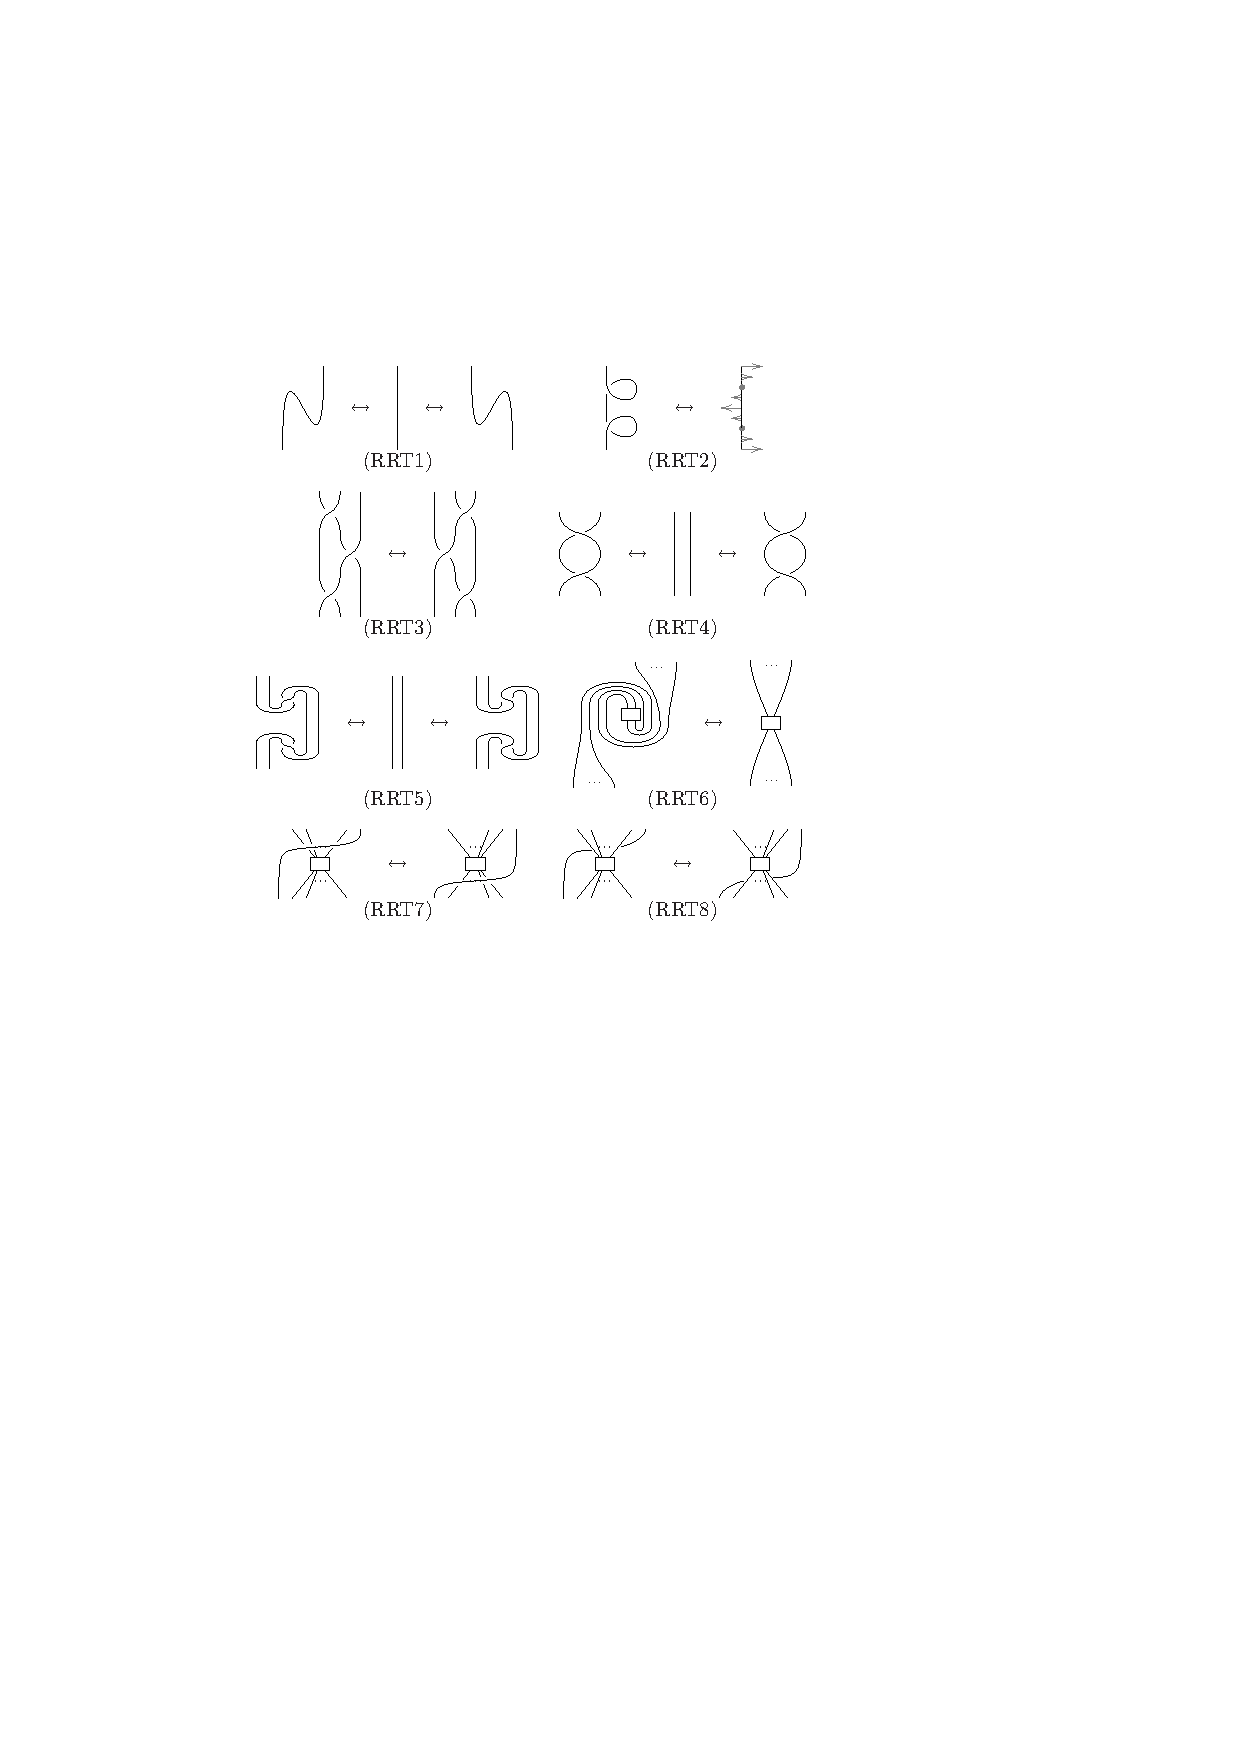
\includegraphics{fig-003}
    \caption{Reidmeister-Reshetikhin-Turaev moves for
      RT-diagrams. Note that move (RRT2) changes a trivial framing
      into a non-trivial (degree $1$) one.}
    \label{fig:rrt}
\end{figure}

It is clear that the operations $\circ$ and $\otimes$ on $\Hom\RTD$ induce
similar composition and tensor product operations on $\Hom\RTE$: any
two RT-graphs can be juxtaposed to form the tensor product $\otimes$ (see
\csref{fig:graph-otimes}) and a pair of graphs with matching input and
output legs can be stacked to form a new RT-graph (see
\csref{fig:graph-composition}).
\begin{lemma}[{\cite[lemmas 5.2 and 5.3]{reshetikhin-turaev;ribbon-graphs}}]
\label{thm:generators}
The set $\Hom\RTE$ of RT-graphs is generated thorugh $\circ$ and $\otimes$ from
the following elementary pieces, modulo the
Reidmeister-Reshetikhin-Turaev relations of \csref{fig:rrt} (an
orientation must be added to each strand!):
\begin{center}
  {%
    \begin{tabular}{cccccc}
      $\xy*!LC\xybox{(0,0);(0,1)**\dir{-}}\endxy$
      &
      $\xy*!LC\xybox{%
        \vcross~{(0,1)}{(1,1)}{(0,0)}{(1,0)}}\endxy$
      &
      $\xy*!LC\xybox{%
        \vcross~{(0,0)}{(1,0)}{(0,1)}{(1,1)}}\endxy$
      &
      $\xy*!LC\xybox{%
        \vloop~{(0,1)}{(1,1)}{(0,0)}{(1,0)}}\endxy$
      &
      $\xy*!LC\xybox{%
        \vloop~{(0,0)}{(1,0)}{(0,1)}{(1,1)}}\endxy$
      &
      $\xy*!LC\xybox{
        (0,1)*+[F]{\ };%
        (-1,0)**\dir{-},(-0.5,0)**\dir{-},%
        (0,0.5)*+{\ldots},(1,0)**\dir{-},%
        (-1,2)**\dir{-},(-0.5,2)**\dir{-},%
        (0,1.5)*+{\ldots},(1,2)**\dir{-},%
        }\endxy$
      \\
      (a) & (b) & (c) & (d) & (e) & (f)
    \end{tabular}
    }
\end{center}
\end{lemma}
A piece of type (a) is called a ``strand''; those of type (b) and (c)
are named ``crossings''; (d) and (e) are the ``coupling'' and the
``Casimir''; (f) is, plainly, a ``vertex''.
\begin{remark} \csref{thm:generators} just states that an
  RT-diagram is a composition of ``rows'' made of pieces of type
  (a)--(f). Generically, such rows will be made of one piece of type
  (b)--(f) padded with a number of strands (a) on the two sides.
\end{remark}

\begin{definition}
  $\RTE$ is the monoidal category whose arrows are elements of
  $\Hom\RTE$ with the composition law and tensor product induced as a
  quotient of $\Hom\RTD$.
\end{definition}
By the arrows-only description of a category (see \csref{cha:arrows}),
we can deduce that objects in $\RTE$ are finite sequences of signs $\pm1$.
Note that, for any such sequence $S$, the set $\RTE(S,S)$ contains the
directed braids group $B_n \ltimes \setZ_2^n$, so any braid is an
isomorphism in $\RTE$.

The category $\RTE$ has duals: for each object $S$, let $\rdl{S}$ be
the sequence obtained from $S$ by flipping it and reversing all the
signs ---for instance, if $S = (+--)$ then $\rdl{S} = (++-)$---; let
$\ev_S: S\otimes\rdl{S} \to I$ be the only graph which connects corresponding
signs in $S$ and $\rdl{S}$ and has only local maxima of the height
function as critical points (see \textsl{(b)} in \csref{fig:struct}),
finally, let $\coev_S : I \to \rdl{S} \otimes S$ be the graph obtained by
flipping $\ev_S$ (see \textsl{(a)} in \csref{fig:struct}).

The category $\RTE$ is balanced by the family of isomorphisms $\theta_S: S
\to S$ defined by requiring that $\theta_{S\otimes T} := \theta_S \otimes \theta_T$ and
that $\theta_{(+)}$ be the straight line $\ell: [0,1] \ni t \mapsto (0,t,0) \in M$
with the degree $1$ framing $N_\ell: [0,1] \ni u \mapsto \exp 2\pi\I u \in
S^1$. (See \textsl{(c)} in \csref{fig:struct}.)

Finally, $\RTE$ is braided by the family of isomorphisms $\tau_{S,T}$
that swap the positions of $S$ and $T$, with directions chosen so to
match the signs on endpoints. (See \textsl{(d)} in
\csref{fig:struct}.)

\begin{figure}[thbp]
  \centering
  \begin{tabular}{cc}
    {\begin{tabular}{cc}
        $\rdl{S} \otimes S$
        &
        $\overbrace{\hspace{1.5cm}}^{\rdl{S}} \hspace{0.5cm}
        \overbrace{\hspace{1.5cm}}^S$
        \\
        ${\xy<0.5cm,0cm>:0, \ar(0,0);(0,3.5) ^{\coev_S} 
          _{\phantom{\coev_S}} \endxy}$
        &
        
\includegraphics[scale=0.5]{coev}
        \\
        $I$
        &
      \end{tabular}}
    &
    {\begin{tabular}{cc}
        $I$
        &
        \\
        $\xy<0.5cm,0cm>:0, \ar(0,0);(0,3.5) ^{\ev_S} _{\phantom{\ev_S}} \endxy$
        &
        
\includegraphics[scale=0.5]{ev}
        \\
        $S \otimes \rdl{S}$
        &
        $\underbrace{\hspace{1.5cm}}_{S} \hspace{0.5cm}
        \underbrace{\hspace{1.5cm}}_{\rdl{S}}$
      \end{tabular}}
    \\
    \textsl{(a)}
    &
    \textsl{(b)}
    \\[12pt]
    {\begin{tabular}{cc}
        S
        &
        S
        \\
        ${\xy<0.75cm,0cm>:0, 
          \ar(0,0);(0,3) ^{\theta_S} _{\phantom{\theta_S}}
          \endxy}$
        &
        ${\xy<1.125cm,0cm>:0,%
          (0,0);(0,2)**\dir{-},
          \ar@[grey] (0,0.00);(+0.50,0.00),
          \ar@[grey] (0,0.25);(+0.25,0.25),
          \ar@{-} (0,0.50)*[grey]{\bullet};(0,0.50),
          \ar@[grey] (0,0.75);(-0.25,0.75),
          \ar@[grey] (0,1.00);(-0.50,1.00),
          \ar@[grey] (0,1.25);(-0.25,1.25),
          \ar@{-} (0,1.50)*[grey]{\bullet};(0,1.50),
          \ar@[grey] (0,1.75);(+0.25,1.75),
          \ar@[grey] (0,2.00);(+0.50,2.00),
          (1,1.5)*{\ldots},
          (2,0);(2,2)**\dir{-},
          \ar@[grey] (2,0.00);(2.50,0.00),
          \ar@[grey] (2,0.25);(2.25,0.25),
          \ar@{-} (2,0.50)*[grey]{\bullet};(2,0.50),
          \ar@[grey] (2,0.75);(1.75,0.75),
          \ar@[grey] (2,1.00);(1.50,1.00),
          \ar@[grey] (2,1.25);(1.75,1.25),
          \ar@{-} (2,1.50)*[grey]{\bullet};(2,1.50),
          \ar@[grey] (2,1.75);(2.25,1.75),
          \ar@[grey] (2,2.00);(2.50,2.00),
          \endxy}$
        \\
        S
        &
        S
      \end{tabular}}
    &
    {\begin{tabular}{cc}
        $T\otimes S$
        &
        $\overbrace{\hspace{1.5cm}}^T \hspace{0.75cm}
        \overbrace{\hspace{1.5cm}}^S$
        \\
        $\xy<0.75cm,0cm>:0, \ar(0,0);(0,3) ^{\tau_{S,T}} _{\phantom{\tau_{S,T}}} \endxy$
        &
        
\includegraphics[scale=0.75]{braid}
        \\
        $S\otimes T$
        &
        $\underbrace{\hspace{1.5cm}}_S \hspace{0.75cm}
        \underbrace{\hspace{1.5cm}}_T$
      \end{tabular}}
    \\
    \textsl{(c)}
    &
    \textsl{(d)}
  \end{tabular}
  \caption{The structure morphisms making $\RTE$ into a braided \textsl{(d)},
    autonomous \textsl{(a, b)}, tortile \textsl{(c)} category. The
    directions on each strand must be chosen according to the signs in
    $S$ and $T$. Note that the balancing $\theta_S$ is just the identity
    with a different framing.}
  \label{fig:struct}
\end{figure}

\begin{proposition}\label{thm:rt}
  The category $\RTE$ is braided, autonomous, and tortile.
\end{proposition}
\begin{proof}
  All the verifications reduce to checking that some RT-graph
  corresponding to a composition of the strcture morphisms is
  \emph{isotopic} to some other RT-graph, again composition of the
  structure morphisms ---for instance, move (RRT1) in \csref{fig:rrt}
  is the verification that $(\ev_{(\pm)}, \coev_{(\pm)})$ is a duality
  pair--- and this is easily done.
\end{proof}


\section{Graphical calculus on tortile braided tensor categories}
\label{sec:rt-gc}
Now let $\A$ be a tensor category. Define $\freemsc{\A}$ to be the
category whose objects are finite sequences $(A_1, \ldots, A_r; \varepsilon_1, \ldots,
\varepsilon_r)$ of objects in $\A$ and signs $\pm1$, whereas a morphism $(A_*,
\varepsilon_*) \to (B_*, \delta_*)$ is an element $f \in \A(A_1^{\varepsilon_1} \otimes \ldots \otimes
A_r^{\varepsilon_r}, B_1^{\delta_1} \otimes \ldots B_s^{\delta_s})$ --- recall that $A^1 = A$
and $A^{-1} = \rdl{A}$.  There is an obvious functor $\freemsc{\A} \to
\A$ defined on objects by $(A_1, \ldots, A_r; \varepsilon_1, \ldots, \varepsilon_r) \mapsto
A_1^{\varepsilon_1} \otimes \cdots \otimes A_r^{\varepsilon_r}$.
\begin{definition}
  An $\A$-colored RT-diagram $\Gamma$ is an RT-diagram together with:
  \begin{enumerate}
  \item an assignment of an object $A_\ell \in \A$ for each
    $\ell\in\Edges{\Gamma}$;
  \item an assignment of a morphism $f\in\A(\Src(v),\Tgt(v))$ for each
    vertex $v$ of $\Gamma$, where $\Src(v)$ and $\Tgt(v)$ are the
    sequences $(A_1, \ldots, A_r;\varepsilon_1, \ldots, \varepsilon_r)$ of objects and signs
    decorating edges in $\In(v)$ and $\Out(v)$.
  \end{enumerate}
  The source and the target of an $\A$-colored RT-diagram are defined
  analogously and are denoted $\Src_\A(\Gamma)$ and $\Tgt_\A(\Gamma)$ respectively.
\end{definition}
It is trivial to generalize \csref{dfn:diagrams-category} to
$\A$-colored RT-diagrams.
\begin{definition}
  The category of $\A$-colored RT diagrams $\RTD[\A]$  has
  $\freemsc{A}$ as its set of objects and $\A$-colored RT-diagrams as
  morphisms. 
\end{definition}
For each $\A$-colored RT-diagram $\Gamma$, $\Src{}_{\A}(\Gamma)$ and
$\Tgt{}_{\A}(\Gamma)$ are objects of $\freemsc{\A}$.  Obviously, $\circ$ and
$\otimes$ are bilinear with respect to the vector space structure on the
$\Hom$-sets of $\RTD[\A]$. Any $\A$-colored RT-diagram can be seen as
the planar projection of an $\A$-colored RT-graph and the following
analogue of lemma \ref{thm:generators} hold.
\begin{proposition}
\label{thm:rt1}
The set $\Hom\RTD[\A]$ of $\A$-colored RT-diagrams is generated thorugh
$\circ$ and $\otimes$ from the following elementary pieces (an orientation
must be added to each strand!):
\begin{center}
  {%
    \begin{tabular}{cccccc}
      $\xy*!LC\xybox{(0,0)*+{A};(0,1)*+{A}**\dir{-}}\endxy$
      &
      $\xy*!LC\xybox{%
        \vcross~{(0,1)*+{B}}{(1,1)*+{A}}{(0,0)*+{A}}{(1,0)*+{B}}}\endxy$
      &
      $\xy*!LC\xybox{%
        \vcross~{(0,0)*+{B}}{(1,0)*+{A}}{(0,1)*+{A}}{(1,1)*+{B}}}\endxy$
      &
      $\xy*!LC\xybox{%
        \vloop~{(0,1)}{(1,1)}{(0,0)*+{A}}{(1,0)*+{A}}}\endxy$
      &
      $\xy*!LC\xybox{%
        \vloop~{(0,0)}{(1,0)}{(0,1)*+{A}}{(1,1)*+{A}}}\endxy$
      &
      $\xy*!LC\xybox{
        (0,1)*+[F]{f};%
        (-1,0)*+{A_1}**\dir{-},(-0.5,0)*+{A_2}**\dir{-},%
        (0,0.5)*+{\ldots},(1,0)*+{A_r}**\dir{-},%
        (-1,2)*+{B_1}**\dir{-},(-0.5,2)*+{B_2}**\dir{-},%
        (0,1.5)*+{\ldots},(1,2)*+{B_s}**\dir{-},%
        }\endxy$
      \\
      (a) & (b) & (c) & (d) & (e) & (f)
    \end{tabular}
    }
\end{center}
The set $\Hom\RTE[\A]$ of $\A$-colored RT-graphs is the quotient of
$\Hom\RTD[\A]$ with respect to the Reidmeister-Reshetikhin-Turaev
relations of \csref{fig:rrt}.
\end{proposition}

Let $\category{B}$ be a tensor category. A tensor functor
$\RTD[\A]\to{\category{B}}$ is uniquely specified if we define it on
the generators; it induces a tensor functor $\RTE[\A] \to \category{B}$
if it is compatible with relations (RRT1)--(RRT8).  In particular,
taking $\category{B}=\A$ we find the following.
\begin{theorem}[Reshetikhin-Turaev,
  \cite{reshetikhin-turaev;ribbon-graphs}]
  \label{thm:rt2}
  For any autonomous balanced braided tensor category $\A$, there is a
  tensor functor $Z_{\A}: \RTD[\A] \to \A$, mapping an object $(A_1,
  \ldots, A_k; \varepsilon_1, \ldots, \varepsilon_k) \in \RTD[\A]$ to $A_1^{\varepsilon_1} \otimes \dots \otimes
  A_k^{\varepsilon_k} \in \A$, and defined on generators of morphisms in
  $\RTD[\A]$ by
\begin{center}
  \everyxy={/r24pt/:}
  {%
    \begin{tabular}{ccc}
      $\xy*!LC\xybox{%
        \vcross~{(0,1)*+{B}}{(1,1)*+{A}}{(0,0)*+{A}}{(1,0)*+{B}}}\endxy
      \mapsto \tau_{XY},$
      %\label{graph-cross+}
      &
      $\xy*!LC\xybox{%
        \vcross~{(0,0)*+{B}}{(1,0)*+{A}}{(0,1)*+{A}}{(1,1)*+{B}}}\endxy
      \mapsto \tau_{XY}^{-1},$
      %\label{graph-cross-}
      &
      $\xy*!LC\xybox{
        (0,1)*+[F]{f};%
        (-1,0)*+{A_1}**\dir{-},(-0.5,0)*+{A_2}**\dir{-},%
        (0,0.5)*+{\ldots},(1,0)*+{A_r}**\dir{-},%
        (-1,2)*+{B_1}**\dir{-},(-0.5,2)*+{B_2}**\dir{-},%
        (0,1.5)*+{\ldots},(1,2)*+{B_s}**\dir{-},%
        }\endxy \mapsto f$
      %\label{graph-morphism} 
      \\
      $\xy*!LC\xybox{%
        \vloop~{(0,1)}{(1,1)}{(0,0)*+{A}}{(1,0)*+{A}}}\endxy \mapsto
      \ev_{A},$
      %\label{graph-casimir}
      &
      $\xy*!LC\xybox{%
        \vloop~{(0,0)}{(1,0)}{(0,1)*+{A}}{(1,1)*+{A}}}\endxy \mapsto
      \coev_{A},$
      %\label{graph-coupling}
      &
      $\xy*!LC\xybox{(0,0)*+{A};(0,1)*+{A}**\dir{-}}\endxy \mapsto
      \id_X,$
      %\label{graph-id}
    \end{tabular}
    }
  \end{center}
where $\tau_{AB}$, $\ev_A$, $\coev_A$ are the structure maps in
$\A$, and $f$ is a morphism in $\A$; take the dual of an
object if the sign $\varepsilon$ on the corresponding edge is $-1$.

The tensor functor $Z_\A$ is invariant by the
Reidmeister-Reshetikhin-Turaev moves (RRT1)--(RRT8), so it induces a
faithful\FIXME{Non sono proprio sicuro che sia fedele!} tortile
braided functor $Z_\A: \RTE[\A] \to \A$.
\end{theorem}
\begin{remark}
By definition of a tensor functor, the following relations hold:
\begin{gather*}
  Z_{\A}(\Gamma\circ\Phi) = Z_{\A}(\Gamma) \circ Z_{\A}(\Phi), 
  \qquad 
  Z_{\A}(\Gamma\otimes\Phi) = Z_{\A}(\Gamma) \otimes Z_{\A}(\Phi),
  \\
  Z_{\A}(a\Gamma + b\Phi) = aZ_{\A}(\Gamma) + bZ_{\A}(\Phi).
\end{gather*}
\end{remark}

%%% Local Variables: 
%%% mode: latex
%%% TeX-master: "index"
%%% x-symbol-8bits: nil
%%% End: 


